\documentclass{paper}

\usepackage{latexsym}
\usepackage{amssymb}
\usepackage{amsmath}
\usepackage{amsfonts}
\usepackage{verbatim}
\usepackage{listings}
\usepackage{graphicx}
\usepackage{float}

\begin{document}

\section{Implement Gradient Descent}

When testing my gradient descent procedure on the function
\[
f(x, y) = x^2 + y^2,
\]
which has gradient
\[
\nabla f(x, y) = [2x, 2y]
\]
with an initial guess of $(x, y) = (3, 5)$, a step size of $0.1$, and a convergence criterion of $10^{-11}$. it returns an answer of $(x_{min}, y_{min}) = (6.17064209 * 10^{-7},   1.02844035 * 10^{-6})$. By inspection, the actual minimum of $f$ occurs at $(0, 0)$. The gradient descent function was close to the correct answer, and can be made arbitrarily closer by lowering the value of the convergence criterion. The convergence criterion is the threshold value $t$ such that the descent algorithm stops running and returns $g_{i+1}$ when $|f(g_i) - f(g_{i+1})| \le t$, where the $g_j$ are successive guesses as to the vector $(x_{min}, y_{min})$.

If lowering the convergence criterion makes the result closer to the true answer, what about changing the step size and the starting guess? Increasing the step size from $0.1$ reduces the error in the answer, up until the step size is $0.5$ - this also decreases the number of iterations that the algorithm needs to run before converging. When the step size is $0.5$ in this example the answer is exactly correct - the algorithm returns $(0, 0)$; increasing the step size any larger causes the algorithm to overshoot the correct answer by an extremely fast-growing amount, and the number of steps required for convergence is very high. Naturally these numbers are unique to this particular example, but the takeaway is that while having a large step size can increase accuracy and convergence speed up to a point, taking steps that are too large can cause incorrect answers and divergent estimates rather than convergent ones.

Increasing the magnitude of the guess by 10 in this example caused the gradient descent procedure to take 10 more iterations, and the number of iterations continues to grow as the guess becomes further from the answer.

While my gradient descent implementation took between 11 and 55 iterations to converge depending on the parameters, the PyLab function \texttt{fmin\_bfgs} was able to converge in 2 iterations with error on the order of $10^{-15}$ in both $x$ and $y$.

My numerical gradient approximation function using central differences returns very accurate answers. The value of $\nabla f(3, 5)$ should be $(6, 10)$; my approximation function returns $(5.999964969305438, 9.999965300266922)$.

\section{Linear Basis Function Regression}

Computing maximum-likelihood weights, and plotting the polynomials given by those weight vectors for orders 0, 1, 3 and 9, results in the following plots, very similar to the graphs in the Bishop text.

\begin{figure}[H]
	%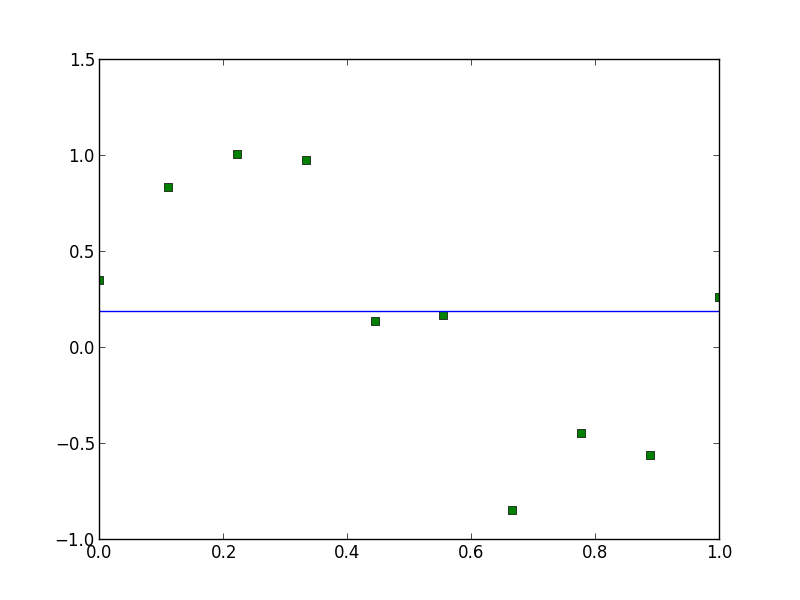
\includegraphics[width=165px]{plot1.png}
	
	%\caption{OLS regression. Fits of order 0 (top left), 1 (top right), 3 (bottom left), 9 (bottom right).}
\end{figure}


When calculating the gradient of the error of these models (evaluated on $w$, the vector of weights), both the analytical function and the numerical gradient function return very similar answers - close to 0. We expect the values to be almost the same, and it makes sense for them both to be close to 0 because the weights were chosen to minimize the error. For examle, in plot number 2 above, the analytically calculated error gradient was $(1.33226763 * 10^{-15}, 1.11022302 * 10^{-15})$, while the numerically calculated gradient was $(4.4408920985006255 * 10^{-11}, 0.0)$.

Setting the step size to 0.01 or 0.02 allows the gradient descent to converge; setting it to 0.1 causes it to wildly diverge. Setting the convergence criterion to $10^{-3}$ causes the algorithm to converge pretty quickly though the fit is not very good. A convergence criterion of $10^{-5}$, however, takes longer but produces a much better fit. PyLab's \texttt{fmin\_bfgs} converges very quickly and produces a good fit.

\section{Ridge Regression}

Upon adding a regularization term to the error function following the ``ridge regression'' technique, overfitting decreased especialy for large values of $M$ (the order of the polynomial used for the fit). Some plots are shown below:

\end{document}

